% pdflatex -jobname="Carolina_Branas_CV" spanish.tex

\documentclass{resume}
\usepackage[left=0.6in,top=0.6in,right=0.6in,bottom=0.55in]{geometry}
\usepackage{vwcol}
\usepackage{natbib}
\setlength{\bibsep}{2.5pt}
\usepackage[svgnames]{xcolor}
\usepackage{hyperref}
\usepackage{graphicx}
\hypersetup{%
  colorlinks=true,
  allcolors=DarkRed,
  pdfborderstyle={/S/U/W 1}
}

\begin{document}

%%%%%%%%%%%%%%%%%%%%%%%%%%%%%%%%%%%%%%%%%%%%%%%%% TÍTULO
\vspace*{-3.5em}

\begin{minipage}[t]{0.72\textwidth}
    \raggedright
    {\Huge \textbf{Carolina Brañas}}\\[0.4em]
    {\normalsize \textbf{Científica de Datos}}\\[0.8em]
    {\small
    A Coruña, España $\bullet$
    (+34) 644 004 477 $\bullet$
    \href{mailto:carobrasor@gmail.com}{carobrasor@gmail.com} \\[0.25em]
    \href{https://carobs9.github.io/}{carobs9.github.io} \\[0.25em]
    \href{https://github.com/carobs9}{github.com/carobs9} \\[0.25em]
    \href{https://www.linkedin.com/in/carolinabranas/}{linkedin.com/in/carolinabranas} \\[0.25em]
    \href{https://huggingface.co/carobs9}{huggingface.co/carobs9}
    }\\[1em]

    {\small
    Soy una científica de datos con experiencia práctica en la construcción de modelos de aprendizaje automático (machine learning) y procesamiento del lenguaje natural (NLP), el diseño de flujos de trabajo de datos escalables y la conversión de datos complejos en información accionable. \\[0.25em]
    Mis intereses incluyen el aprendizaje automático, el análisis de redes, el procesamiento del lenguaje natural y los datos geoespaciales. 
    }
\end{minipage}%
\hfill
\begin{minipage}[t]{0.23\textwidth}
    \vspace*{0.3em}  % small downward shift so it doesn't hit the margin
    \begin{flushright}
        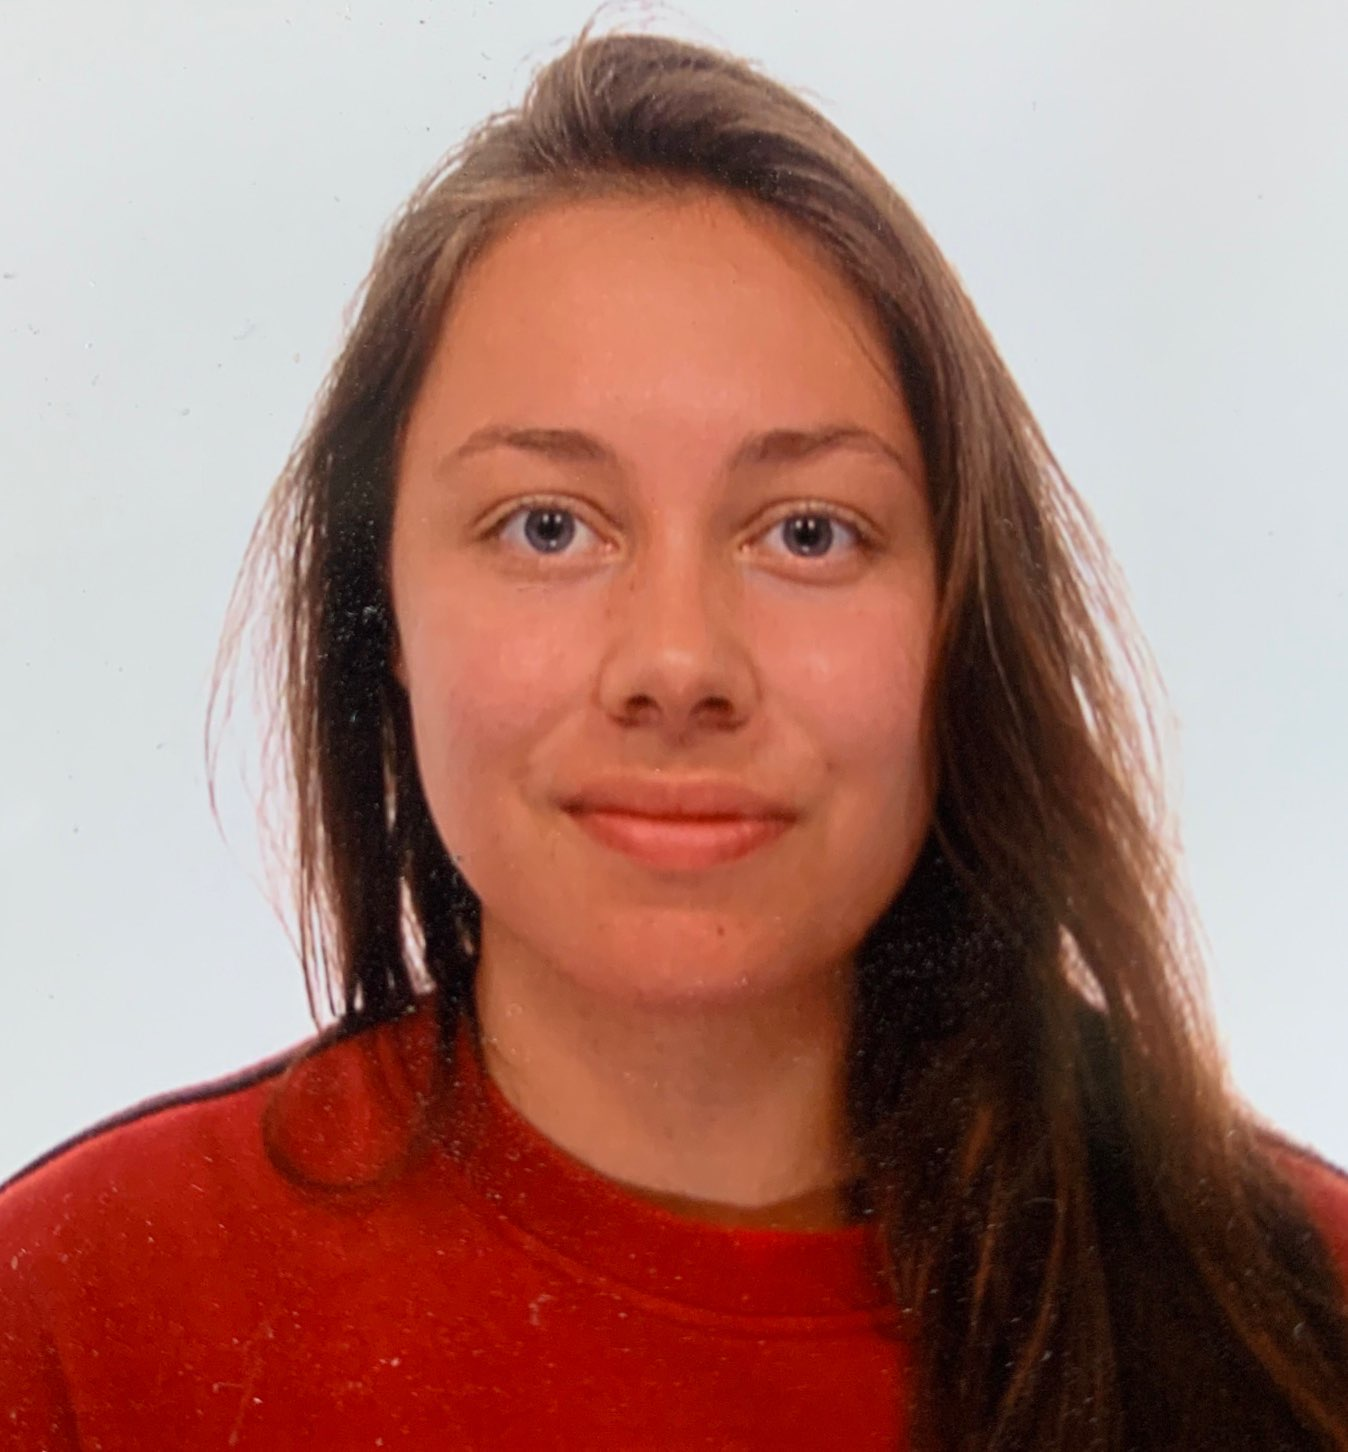
\includegraphics[width=3cm,clip,trim=0 0 0 0]{profile.jpg}
    \end{flushright}
\end{minipage}

%%%%%%%%%%%%%%%%%%%%%%%%%%%%%%%%%%%%%%%%%%%%%%%%% EXPERIENCIA
\section{EXPERIENCIA}
\begin{content}

    \begin{position}{Asistente de Investigación, Ciencia de Datos}{Mayo 2024 -- Presente}{Universidad de Copenhague, Dinamarca}{Prof.~Jeanet Bentzen}{}
        \item Contribuí al proyecto de investigación {\href{https://www.economics.ku.dk/research/externally-funded-research_new/shocking-religion/}{Shocking Religion}} sobre el impacto económico de la religión.
        \item Desarrollé modelos de temas para descubrir tendencias temáticas en datos textuales.
        \item Creé flujos de trabajo basados en LLM y RAG para la extracción de información en documentos.
        \item Diseñé y contenedoricé flujos de trabajo de datos escalables (Docker); gestioné la ingesta y el preprocesamiento de datos a gran escala; desplegué soluciones en infraestructura en la nube (UCloud).
        \item Trabajé con un equipo de investigación multidisciplinar.
    \end{position}
    
    \begin{position}{Científica de Datos}{Octubre 2023 -- Mayo 2024}{Above Sports, Dinamarca}{}{ }
        \item Automatizé flujos de trabajo de datos para mejorar la eficiencia.
        \item Desarrollé modelos de computer vision para detección de logotipos de marca en vídeo.
        \item Colaboré con equipos de producto para refinar la calidad de los resultados.
        \item Dockericé soluciones para flujos de trabajo escalables y reproducibles.
    \end{position}
    
    \begin{position}{Estratega de Marketing}{Septiembre 2021 -- Mayo 2022}{Crescendo Collective, Estados Unidos}{}{ }
        \item Analicé datos de campañas mediante Google Analytics; gestioné informes y estrategias de Google Ads.
        \item Automatizé informes internos con scripts en Python.
        \item Realicé análisis de competencia y comparativas.
        \item Colaboré con el equipo de datos para obtener información sobre audiencias; presenté informes a clientes.
    \end{position}
    
\end{content}

%%%%%%%%%%%%%%%%%%%%%%%%%%%%%%%%%%%%%%%%%%%%%%%%% EDUCACIÓN 
\section{EDUCACIÓN} 
\begin{content}
    {\bf M.Sc. en Ciencia de Datos Sociales} \hfill {\bf 2022 -- 2024} \\ 
    Universidad de Copenhague, Dinamarca \\ 
    {\bf \em Tesis:} {\href{https://github.com/carobs9/segregation-madrid}{Movilidad y segregación por ingresos en Madrid, España.}} \\ 
    {\em Cursos Optativos:} \\ 
    {\small
    Aprendizaje Automático Avanzado para Ciencia de Datos (IT University of Copenhagen) \\ 
    Ciencia de Datos Geoespaciales (IT University of Copenhagen) \\ 
    Ciencia de Redes Avanzada (IT University of Copenhagen) \\ 
    Procesamiento del Lenguaje Natural (Departamento de Ciencias de la Computación, DIKU) \\ 
    }

    {\bf B.Sc. en Marketing, Minor en Ingeniería Informática} \hfill {\bf 2018 -- 2022} \\ 
    Cardinal Stritch University, Estados Unidos \\ 
    {\em Honores:} Magna Cum Laude, Lista del Decano (2018--2022), Mejor Promedio del Grado en Marketing (2022)
\end{content}

%%%%%%%%%%%%%%%%%%%%%%%%%%%%%%%%%%%%%%%%%%%%%%%%% IDIOMAS 
\section{IDIOMAS} 
\begin{content}
    {\bf Español:} Nativo \\ 
    {\bf Gallego:} Nativo \\ 
    {\bf Inglés:} Competencia Profesional \\ 
    {\bf Portugués:} Principiante \\
\end{content}

%%%%%%%%%%%%%%%%%%%%%%%%%%%%%%%%%%%%%%%%%%%%%%%%% HABILIDADES 
\section{HABILIDADES} 
\begin{content}
    {\bf Programación y Procesamiento de Datos:} Python {\footnotesize (pandas, numpy, matplotlib, tensorflow, pytorch, scikit-learn)}, SQL, Bash \\ 
    {\bf Aprendizaje Automático y NLP:} Transformers, Topic Modeling {\footnotesize (UMAP, HDBSCAN, BERTopic)}, Hugging Face, Weights and Biases, Deep Learning, Modelos Predictivos, Computer Vision \\ 
    {\bf Visualización y Análisis de Datos:} Matplotlib, Seaborn, Tableau, Power BI, Análisis Estadístico, Limpieza de Datos \\ 
    {\bf Geoespacial:} Geopandas, Rasterio, QGIS, Análisis Geoespacial \\ 
    {\bf Cloud y DevOps:} Docker, Git, Linux, VSCode, AWS, UCloud, CI/CD \\
    {\bf Otros:} \LaTeX, Overleaf, Estadística \\
\end{content}

%%%%%%%%%%%%%%%%%%%%%%%%%%%%%%%%%%%%%%%%%%%%%%%%% PREMIOS
\section{PREMIOS}
\begin{content}
    \prize{Lista del Decano}{2018--2022}{Reconocida en la Lista del Decano cada semestre por mantener un GPA superior a 3.5 sobre 4.0 con al menos 12 créditos.} \\ 
    \prize{Mejor Promedio del B.Sc. en Marketing}{2022}{Graduada con el promedio más alto de la carrera de Marketing con Ingeniería Informática en la promoción 2022.} \\ 
    \prize{Beca Académica y Deportiva}{2018--2022}{Beca completa otorgada por excelencia académica y rendimiento en fútbol durante cuatro años.}
\end{content}

\end{document}
